\chapter{Implementation}  
\label{cha:implementation}

% Say something about implementation without showing the code, maybe giving pseudocode. Talk about distance between formalization and implementation. Describe examples, error messages, practical applications, how it can be used, how it detects paradoxes, how warnings can be given to users.
In this chapter, we present the implementation. We first give an overview of the types to display the structure of the implementation. An example is presented to show how it looks in practice. We also briefly present the translation of the analysis rules, and give an example of an application.


\section{Overview}
\label{sec:overview}
We have created a prototype for an implementation of the analysis rules. The implementation can be found on GitHub\footnote{\url{https://github.com/idamotz/Master/tree/master/soundness-checker}}. The implementation is not meant to be integrated directly into a tool, but serves as a proof of concept that our analysis method is realisable in practice. It can also serve as a guide for how to interpret the rules where they are unclear, if they are to be realised as part of a SPL planning tool. 

The prototype is implemented in Haskell\footnote{\url{https://www.haskell.org/}}, which is a strongly typed, purely functional programming language. We chose the language since a functional language corresponds closely to the mathematical nature of our analysis rules. Moreover, Haskell has an implementation of interval maps\footnote{\url{https://hackage.haskell.org/package/IntervalMap}} which are easily adapted to our purposes. 

The most important modules are \texttt{Types},
% \texttt{Helpers}, TODO: review if there should be a section on this or just mention it in passing
\texttt{Validate}, and \texttt{Apply}. We give brief introductions to these modules in the following sections. 

\subsection{Translation from Definitions to Types}
\label{sub:the-types-module}

In the \texttt{Types} module we define all the types used throughout the project, corresponding closely with our definitions (see Chapter~\vref{cha:basics}). Our time points are implemented as an abstract data type \texttt{TimePoint}. The possible \texttt{TimePoints} are \texttt{TP n}, where \texttt{n} is an integer, or \texttt{Forever}, which corresponds to $\forever$. For all integers \texttt{n}, we have that \texttt{TP n < Forever}. Our notion of intervals are translated to an abstract data type \texttt{Validity}. Using
\begin{minted}{haskell}
   Validity (TP 3) (TP 5)
\end{minted}
gives us the interval $\interval{3}{5}$. Similarly, \texttt{Validity (TP 1) Forever} corresponds to the interval $\interval{1}{\forever}$. 

We base our implementation of the interval maps on the Haskell module \texttt{Interval\-Map}. To customise it to our needs, we name our representation \texttt{Validity\-Map}, specifying that the keys are \texttt{Validity}s. The \texttt{IntervalMap} module provides several useful functions, such as \texttt{containing}, which takes an \texttt{Interval\-Map} and a \texttt{Time\-Point} and returns all the keys containing the given time point.

We further define the data type \texttt{Interval\-Based\-Feature\-Model}, which takes the root ID of the IBFM, a \texttt{Name\-Validities} map, a \texttt{Feature\-Validities} map, and a \texttt{Group\-Validities} map. This corresponds closely to our interval-based feature model  $(\nobreak \names,\,\features,\, \groups)$ (see Definition~\vref{def:interval-based-feature-model}). The $\texttt{Name\-Validities}$ map is a Haskell \texttt{Map}\footnote{\url{https://hackage.haskell.org/package/containers-0.4.0.0/docs/Data-Map.html}} from \texttt{Name}, which is a \texttt{String}, to \texttt{Validity\-Map FeatureID}, where \texttt{FeatureID} is a wrapper type for \texttt{String}. Recall from Section~\ref{sec:interval-based-feature-model} that our $\names{}$ map is a map from names to interval maps with feature ID values, which resembles our implementation. The \texttt{Feature\-Validities} map has \texttt{Feature\-ID} keys and \texttt{Feature\-Validity} values. The \texttt{Feature\-Validity} resembles our feature entries $\feature{}$. The interval set $F_e$ is represented by a \texttt{Validity\-Map ()}. The special type \texttt{()} (\emph{unit}) has only one value, namely \texttt{()}. This lets us treat the \texttt{Validity\-Map ()} as an interval map or an interval set (where the interval keys are the elements of the set), depending on our needs. The names map $F_n$ is represented by a \texttt{Validity\-Map Name}, the types map $F_t$ by a \texttt{Validity\-Map Feature\-Type}, the parent group map $F_p$ by a \texttt{Validity\-Map Group\-ID}, and the child group map $F_c$ by a \texttt{Validity\-Map (Set\footnote{\url{https://hackage.haskell.org/package/containers-0.6.4.1/docs/Data-Set.html}} Group\-ID)}.

A group $\group{}$ is defined in much the same way, with a \texttt{Validity\-Map ()} for its existence interval set $G_e$, a \texttt{Validity\-Map Group\-Type} for its types map $G_t$, a \texttt{Validity\-Map Feature\-ID} for its parent feature map $G_p$, and a \texttt{Validity\-Map (Set Feature\-ID)} for its child feature map $G_c$. 

\begin{figure}
   \centering
      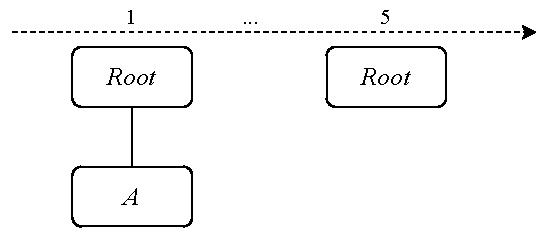
\includegraphics[width=0.6\textwidth]{SimpleParadox1}
   \caption{Simple plan}
   \label{ex:simple-plan}
\end{figure}

The example in Figure~\vref{ex:simple-plan} is formalized below in our previously defined representation, with only one feature (ID feature:root) and one group (ID group:A).

\begin{align*}
 ( \{ \; & \mapping{\text{Root}}{\intervalmapping{1}{\forever}{\text{feature:root}}} \} \\
    \\
    ,\{\; & \mapping{\text{feature:root}}{( \\
          & \{ \interval{1}{\forever}\} ,\, \\
          & \{\intervalmapping{1}{\forever}{\text{Root}}\} ,\, \\
          & \{\intervalmapping{1}{\forever}{\mandatory{}}\} ,\, \\
          &  \emptyset ,\, \\ 
          & \{\intervalmapping{1}{5}{\text{group:A}}\} ) } \\
       \} &\\
          \\
            ,\; \{ \; & [ \text{group:A} \mapsto ( \\
                      & \{\interval{1}{5}\} ,\, \\
                      & \{\intervalmapping{1}{5}{\andtype{}}\} ,\, \\
                      & \{\intervalmapping{1}{5}{\text{feature:root}}\} ,\, \\
                      & \emptyset ) ]\\
 \}&)\\
\end{align*}

Below, the above example is translated to our Haskell representation\footnote{This example can be found in the GitHub repository, in \texttt{soundness-checker/\allowbreak src/\allowbreak SimpleExample.hs}}.

\begin{minted}{haskell}
im :: Validity -> a -> ValidityMap a
im = IM.singleton

simplePlan :: IntervalBasedFeatureModel
simplePlan =
  IntervalBasedFeatureModel
    (FeatureID "feature:root")
    [
      ( "Root"
      , im (Validity (TP 1) Forever) (FeatureID "feature:root")
      )
    ]
    [
      ( FeatureID "feature:root"
      , FeatureValidity
          (im (Validity (TP 1) Forever) ())
          (im (Validity (TP 1) Forever) "Root")
          (im (Validity (TP 1) Forever) Mandatory)
          mempty
          (im (Validity (TP 1) (TP 5)) [GroupID "group:A"])
      )
    ]
    [
      ( GroupID "group:A"
      , GroupValidity
          (im (Validity (TP 1) (TP 5)) ())
          (im (Validity (TP 1) (TP 5)) And)
          (im (Validity (TP 1) (TP 5)) (FeatureID "feature:root"))
          mempty
      )
    ]

\end{minted}

The operations are interpreted quite directly, in two categories: The \texttt{Add\-Operation}s, which take a \texttt{Validity} (interval) and an operation, and the \texttt{Change\-Operation}s, which take a \texttt{TimePoint} and an operation. An operation in general is called a \texttt{Time\-Operation}. To express $\textbf{addFeature}(\text{feature:B}, \text{B}, \mandatory{}, \text{group:A}) \text{ from } 3 \text{ to } \forever$, we write
\begin{minted}[escapeinside=,breaklines]{haskell}
op =
   AddOperation (Validity (TP 3) Forever)
    (AddFeature (FeatureID "feature:B") "B" Mandatory (GroupID "group:A"))
\end{minted}


\subsection{Interpreting the Rules as Code}
Each rule consists of a set of premises, and a conclusion which takes a state and returns a new state. In the implementation, we have chosen to split these up, with one function for verifying the premises, and one for applying the operations.

The \texttt{Validate} module exports only the function \texttt{validate}, which takes a \texttt{Time\-Operation} and an \texttt{Interval\-Based\-Feature\-Model}. The most important difference between this function and the rules is that the function returns a list of errors if paradoxes occur. These errors belong to the type \texttt{Validation\-Error}, and consists of errors like \texttt{Incompatible\-Types}, to be returned if a feature and its parent group have incompatible types, \texttt{Name\-In\-Use}, if a feature is trying to use a name which already belongs to another feature, etc. This is done to show that the cause of a paradox can be located quite precisely.

To apply the operations, the \texttt{Apply} module exports the function \texttt{apply}, which takes a \texttt{Time\-Operation} and an \texttt{Interval\-Based\-Feature\-Model} and applies the operation to the model. This function works similarly to how it is defined in the rules.

The functions are combined in \texttt{validate\-And\-Apply}, which has the return type \texttt{Either [Validation\-Error] Interval\-Based\-Feature\-Model}. If validation fails, it returns a list of errors, and if it succeeds, it applies the operation and returns the modified model.
\begin{figure}
   \centering
      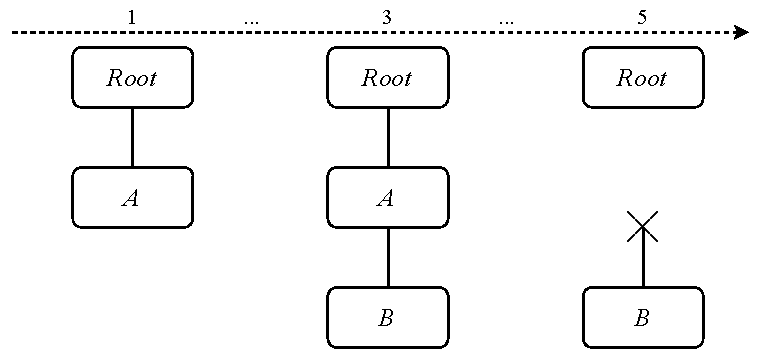
\includegraphics[width=0.7\textwidth]{SimpleParadox2}
   \caption{Illustration of the paradox}
   \label{ex:simple-plan2}
\end{figure}
If we call \texttt{validateAndApply op simplePlan}, where \texttt{op} and \texttt{simplePlan} are defined above, we get the following result:
\begin{minted}[breaklines]{haskell}
Left [ParentNotExists] 
   :: Either [ValidationError] IntervalBasedFeatureModel
\end{minted}
The list of errors, containing \texttt{Parent\-Not\-Exists}, is wrapped in a \texttt{Left} to show that the type is a \texttt{Validation\-Error}. If the operation did not result in an error, we would get a result on the form \texttt{Right ibfm}, where \texttt{ibfm} is an \texttt{Interval\-Based\-Feature\-Model}. The error here means that we are trying to add a feature, but the feature's parent does not exist at some point during the specified interval. In the eample, the parent group \texttt{group:A} is removed at 5, so the feature will be without a parent at that time. The paradox is visualised in Figure~\vref{ex:simple-plan2}.

